\documentclass[10pt]{article}

\usepackage[margin=1.05in]{geometry}
\usepackage{amsmath, amssymb, amsthm}
\usepackage{booktabs}
\usepackage{graphicx}
\usepackage{siunitx}
\usepackage{microtype}
\usepackage[hidelinks]{hyperref}
\usepackage{float}
\usepackage{caption}
\captionsetup{font=small, labelfont=bf}

\newtheorem{proposition}{Proposition}
\newcommand{\diag}{\operatorname{Diag}}
\newcommand{\KL}[2]{D_{\mathrm{KL}}\!\left(#1 \,\middle\|\, #2\right)}
\newcommand{\E}{\mathbb{E}}
\newcommand{\R}{\mathbb{R}}

\title{\textbf{yx49k: Hybrid Gated-Delta-Attention Language Models on
TPU v4 --- a 308M Text Program and a 1B Multimodal Program}}
\author{David-Franco Buga (Yxanul)\\
\small\texttt{github.com/yxanul} $\cdot$ \texttt{huggingface.co/Yxanul}}
\date{August 2026}

\begin{document}
\maketitle

\begin{abstract}
We describe the complete construction of a 307.7M-parameter hybrid
language model trained end-to-end on TPU Research Cloud hardware: a
gated-delta-attention (KDA) architecture with per-channel decay
interleaved 3:1 with NoPE global attention; custom fused Pallas training
kernels built around a chunkwise WY representation, a divide-and-conquer
nilpotent inverse, and an overflow-bounded decay factorization that turns
the gate's lower bound into a kernel compute parameter; a
precision policy qualified against fp64 on real text; a matrix/scalar
split optimizer with orthogonalized updates and a logit-growth guard; and
a 49{,}152-token tokenizer constructed as an exact subset projection of a
4B-parameter teacher's vocabulary, which later makes logit distillation
alignment-free by construction. The model was pretrained on 367B tokens
of ClimbMix on a 32-chip TPU v4-64 at a median 1.09M tokens/s, surviving
a mid-anneal crash with a verified clean resume. At 0-shot it reaches
HellaSwag 56.9, PIQA 75.2, ARC-e 67.5, and WinoGrande 59.4 --- ahead of a
same-size reference model trained on 11$\times$ more tokens on every
comparable benchmark. A post-training stage of supervised fine-tuning
plus offline top-$K$ logit distillation lifts instruction following to
IFEval 51.0, above both major same-size instruction-tuned references when
all models are measured under an identical harness. We close with a
measured attribution of what remains: capability favors our base;
decode-time discipline favors the references' deeper post-training; and
the failure signature identifies on-policy distillation as the indicated
next stage.
Part II scales the recipe to a 0.98B-parameter model with a
from-scratch vision tower trained jointly under the next-token
objective across two campaigns totalling 55B tokens of a calibrated
image/text/code/mathematics mixture. At a fraction of the text budget
the multimodal model matches or exceeds the 308M program's language
benchmarks, grounds vision on held-out data, and --- sharing the same
tokenizer --- accepts the full post-training stack unchanged,
surpassing every Part~I checkpoint on instruction following and answer
quality within a single day of post-training.
\end{abstract}

\tableofcontents

\part{A 308M Text Program}

\section{Introduction}

This report documents a complete small-language-model program carried out
on TPU Research Cloud hardware between 2026-07-20 and 2026-08-08: kernel
development on a single-host TPU v6e-8, a 367B-token pretraining campaign
on a 32-chip TPU v4-64, and a post-training stage (supervised fine-tuning
plus offline logit distillation) evaluated against the strongest publicly
available models of the same size class, all measured under one harness.

The program's through-line is that every layer of the stack was
co-designed with the ones above and below it. The architecture's gate
bound is also the kernel's floating-point overflow budget
(\S\ref{sec:kernels}). The tokenizer is not merely small; it is an exact
subset projection of a 4B teacher's vocabulary, which later deletes an
entire class of distillation alignment machinery
(\S\ref{sec:tokenizer}, \S\ref{sec:posttraining}). The optimizer's
logit-growth guard is priced at zero because its trigger never fired in
700{,}000 steps --- a fact we can state only because the training loop
recorded per-head maximum logits the whole way (\S\ref{sec:optimizer}).

\paragraph{Contributions.}
\begin{enumerate}
  \item A hybrid gated-delta-attention (KDA) model,
  \texttt{kda\_hybrid\_yx49k\_l20}: 307{,}698{,}680 parameters, 20 layers
  as five \([\mathrm{KDA},\mathrm{KDA},\mathrm{KDA},\mathrm{GQA}]\)
  cycles, trained at sequence length 2048 (\S\ref{sec:architecture}).
  \item Fused TPU training kernels for KDA built on a chunkwise WY form:
  a divide-and-conquer explicit inverse that is exact by nilpotency, a
  decay-anchored dot-product factorization with a provable fp32 overflow
  bound, and a split-backward variant for the older v4 ISA
  (\S\ref{sec:kernels}), with a numerics policy qualified against fp64 on
  real text (\S\ref{sec:numerics}).
  \item A matrix/scalar split optimizer --- orthogonalized momentum for
  matrices, AdamW for the rest --- with a grouped-query adaptation of
  attention-logit clipping (\S\ref{sec:optimizer}).
  \item The yx49k tokenizer: 49{,}152 tokens, each mapping to a distinct
  token of the teacher vocabulary, at practical parity with a
  2.6$\times$ larger reference tokenizer on bytes-per-token
  (\S\ref{sec:tokenizer}).
  \item The campaign itself: 700k steps at 524{,}288 tokens per step on
  32 chips, median 1.09M tokens/s, a mid-anneal crash with a
  measurably clean resume, and a terminal anneal worth $-0.195$ nats of
  holdout loss (\S\ref{sec:pretraining}, \S\ref{sec:evaluation}).
  \item A post-training arc --- SFT at 6.27M rows, then offline top-$K$
  logit distillation from a frozen 4B teacher --- with every design
  decision A/B-measured, including a clean null result on repeated
  epochs (\S\ref{sec:posttraining}), and an external calibration against
  Gemma~3 270M IT and SmolLM 360M v1/v2 under identical measurement
  (\S\ref{sec:calibration}).
\end{enumerate}

\begin{table}[h]
\centering
\small
\caption{Summary card.}
\label{tab:summary}
\begin{tabular}{ll}
\toprule
Parameters & 307{,}698{,}680 (tied embeddings) \\
Layers & 20 = 5 $\times$ [KDA, KDA, KDA, GQA], $d_{\mathrm{model}}=1024$ \\
Tokenizer & yx49k (49{,}152 BPE, exact teacher subset) \\
Pretraining data & ClimbMix, 367B step-tokens ($\sim$341B unique) \\
Hardware & TPU v4-64: 32 chips / 8 hosts, pure data parallel \\
Throughput & median 1.09M tokens/s (480 ms / 524{,}288-token step) \\
Final loss & train 2.3617, holdout 2.3494 (ppl 10.48) \\
0-shot & HellaSwag 56.9, PIQA 75.2, ARC-e 67.5, WinoGrande 59.4 \\
Post-training & IFEval mean 51.0 (GOLD mix300k checkpoint) \\
\bottomrule
\end{tabular}
\end{table}

\section{Model architecture}
\label{sec:architecture}

\subsection{Gated delta attention with per-channel decay}

The sequence mixer used in three of every four layers is a linear
attention layer whose state update follows the \emph{delta rule}: rather
than accumulating outer products indiscriminately, each write first
subtracts what the state already predicts for the incoming key. With a
scalar forgetting factor this is
\begin{equation}
S_t \;=\; \alpha_t \left(I - \beta_t k_t k_t^{\top}\right) S_{t-1}
\;+\; \beta_t k_t v_t^{\top},
\qquad o_t = S_t^{\top} q_t ,
\label{eq:scalar-delta}
\end{equation}
where $S_t \in \R^{d_k \times d_v}$ is a per-head fast-weight matrix,
$\beta_t \in (0,1)$ a learned write strength, and $\alpha_t \in (0,1]$ a
learned decay. KDA generalizes the decay from a scalar to a
\emph{per-channel} vector $\alpha_t \in (0,1]^{d_k}$:
\begin{equation}
\boxed{\;
S_t \;=\; \left(I - \beta_t k_t k_t^{\top}\right) \diag(\alpha_t)\,
S_{t-1} \;+\; \beta_t k_t v_t^{\top},
\qquad o_t = S_t^{\top} q_t .
\;}
\label{eq:kda}
\end{equation}
Each key channel now has its own forgetting timescale, so one head can
simultaneously hold long-lived and rapidly-refreshed features. This is
the modeling win that motivates the entire kernel effort of
\S\ref{sec:kernels}: per-channel decay breaks the algebraic shortcuts
available to scalar-decay linear attention, and the training-time
chunkwise form must track a full decay \emph{profile} per position.

\subsection{The bounded gate}

The decay is produced in log space by a low-rank head with a hard lower
bound. With $A = \exp(A_{\log}) \in \R^{H}$ a per-head positive rate and
$f(x) = W^{\uparrow}(W^{\downarrow} x) + b_{dt}$ a rank-128 projection of
the token's hidden state,
\begin{equation}
\log \alpha_t \;=\; g_t \;=\; \ell \,\cdot\, \sigma\!\big(A \odot f(x_t)\big),
\qquad \ell = -5,
\label{eq:safe-gate}
\end{equation}
so that $g_t \in (-5, 0)$ always. An unbounded softplus form
$g_t = -A\,\mathrm{softplus}(f(x_t))$ is implemented as an alternative,
but the bounded form is required by the production kernel: the bound
$|g| < 5$ is exactly what makes the kernel's decay-factorized dot
products representable in fp32 (\S\ref{sec:pairwise}). The write
strength is a per-head scalar $\beta_t = \sigma(w_\beta^{\top} x_t)$.

\subsection{The full layer}

Around the recurrence, the layer applies a fused QKV projection, a
short causal depthwise convolution (width $w{=}4$, one filter per
channel) with a SiLU activation,
\begin{equation}
\tilde{x}_t = \mathrm{silu}\!\Big(\textstyle\sum_{j=0}^{w-1}
W^{\mathrm{conv}}_j \odot x_{t-(w-1)+j}\Big),
\qquad (q_t, k_t, v_t) = \mathrm{split}(\tilde{x}_t),
\end{equation}
then $\ell_2$-normalizes $q$ and $k$ per head
($\hat{u} = u / \max(\lVert u \rVert_2, \varepsilon)$, with
$q \leftarrow \hat{q}/\sqrt{d_k}$), runs \eqref{eq:kda}, and finishes
with a per-head RMSNorm modulated by a learned low-rank output gate:
\begin{equation}
y_t = W_o\left(\mathrm{RMSNorm}(o_t) \odot
\sigma\!\big(W_g^{\uparrow} (W_g^{\downarrow} x_t) + b_g\big)\right).
\end{equation}
Heads are $H = 8$ with $d_k = d_v = 128$.

\subsection{The hybrid stack}

Layers are arranged in cycles of four --- three KDA layers followed by
one full-attention layer --- repeated five times for the 20-layer model.
The global layer is grouped-query attention (8 query heads, 2 KV heads,
$d_h = 128$) with \emph{no positional encoding} (NoPE): position
information reaches it only through the recurrent layers below and the
causal convolutions, which measurably suffices at this scale and keeps
the decode-time KV cache free of any position-dependent transform. The
channel mixer everywhere is a fused SwiGLU MLP,
$\mathrm{MLP}(x) = W_o\big(\mathrm{silu}(W_1 x) \odot W_2 x\big)$ with
inner width 2816; normalization is pre-norm RMSNorm
($\varepsilon = 10^{-5}$, no centering, no bias); the output head is
tied to the input embedding. Cycles are scanned with parameters stacked
along a scan axis, and rematerialization operates per cycle.

\begin{table}[h]
\centering
\small
\caption{\texttt{kda\_hybrid\_yx49k\_l20} hyperparameters.}
\label{tab:hparams}
\begin{tabular}{llll}
\toprule
vocabulary & 49{,}152 & layers & 20 (5 cycles) \\
$d_{\mathrm{model}}$ & 1024 & cycle & [KDA, KDA, KDA, GQA] \\
MLP inner & 2816 (SwiGLU) & norm & RMSNorm, $\varepsilon{=}10^{-5}$ \\
KDA heads & 8 $\times$ ($d_k{=}d_v{=}128$) & conv width & 4 \\
gate & rank 128, $\ell = -5$ & $q,k$ & $\ell_2$-normalized \\
GQA heads & 8 query / 2 KV, $d_h{=}128$ & positions & NoPE \\
embeddings & tied & sequence & 2048 \\
precision & bf16 compute, fp32 master & params & 307{,}698{,}680 \\
\bottomrule
\end{tabular}
\end{table}

Parameter accounting: the tied embedding contributes
$49{,}152 \times 1024 = 50.3$M; each cycle carries three KDA mixers,
one GQA mixer, four SwiGLU blocks, and their norms; five cycles plus the
final norm bring the total to 307{,}698{,}680. Relative to same-size
references, the small vocabulary shifts roughly 25M parameters from the
embedding table into the transformer body --- a deliberate exchange of
rare-token coverage for depth-adjusted compute, made survivable by the
tokenizer's byte-level fallback (\S\ref{sec:tokenizer}).

\section{Chunkwise WY form and the TPU kernels}
\label{sec:kernels}

Equation~\eqref{eq:kda} is a sequential recurrence; trained naively it
serializes 2048 steps. The training path instead processes the sequence
in chunks of $C = 64$, expressing everything inside a chunk with dense
matrix algebra (which TPUs execute at full matrix-unit utilization) and
carrying the fast-weight state only across chunk boundaries.

\subsection{Chunkwise decomposition}

Write $G_i = \sum_{s \le i} g_s \in \R^{d_k}$ for the inclusive
cumulative log-decay within a chunk. Unrolling \eqref{eq:kda} from the
chunk-entry state $S$ gives, for the output at intra-chunk position $i$,
a \emph{cross-chunk} term read through the accumulated decay and an
\emph{intra-chunk} term over earlier positions of the same chunk:
\begin{equation}
o_i \;=\; \big(q_i \odot e^{G_i}\big)^{\top} S
\;+\; \sum_{j \le i} \Xi_{ij}\, \hat{v}_j,
\qquad
\Xi_{ij} = \big\langle q_i \odot e^{G_i - G_j},\, k_j \big\rangle ,
\label{eq:chunk-out}
\end{equation}
where the $\hat{v}_j$ are \emph{delta-corrected} values: the values
actually written to the state after subtracting the state's own
prediction. The corrections inside one chunk satisfy a unit-lower-
triangular linear system. Defining the decay-weighted Gram matrix
$M_{ij} = \langle \beta_i k_i \odot e^{G_i - G_j},\, k_j\rangle$ for
$j < i$ and $T = \mathrm{StrictLower}(M)$,
\begin{equation}
(I + T)\, U = B_v, \qquad (I + T)\, W = B_k,
\label{eq:wy-solve}
\end{equation}
with $B_v = [\beta_i v_i]_i$ and $B_k = [\beta_i k_i \odot e^{G_i}]_i$.
This is the WY representation of the product of rank-one delta updates:
$U$ and $W$ compress the chunk's 64 sequential writes into two dense
matrices. The corrected values and the state advance are then
\begin{equation}
\hat{V} = U - W S,
\qquad
S \leftarrow \diag\!\big(e^{G_C}\big)\, S
+ \big(k \odot e^{G_C - G}\big)^{\top} \hat{V},
\label{eq:chunk-scan}
\end{equation}
one dense contraction per chunk, with $S$ the only sequential carrier.

\subsection{Decay-anchored pairwise dots and the overflow bound}
\label{sec:pairwise}

Every matrix above contains entries of the form
\begin{equation}
M_{ij} \;=\; \sum_{d} L_{i,d}\, R_{j,d}\, e^{G_{i,d} - G_{j,d}},
\label{eq:pairwise}
\end{equation}
which cannot be computed as a plain matmul because the decay factor
depends on \emph{both} indices and on the channel. Materializing the
$[C, C, d_k]$ tensor is prohibitive; factorizing
$e^{G_i - G_j} = e^{G_i} e^{-G_j}$ overflows, since $-G_j$ can reach
$|\ell| \cdot C = 320$ and $e^{320}$ is far beyond fp32.

The kernel factorizes against a moving \emph{anchor} instead. Rows are
processed in blocks of $R$ rows; each block is anchored at its last
row's cumulative decay $a = G_{\text{block end}}$:
\begin{equation}
M_{ij} = \sum_d
\underbrace{\big(L_{i,d}\, e^{G_{i,d} - a_d}\big)}_{\text{left factor}}
\cdot
\underbrace{\big(R_{j,d}\, e^{a_d - G_{j,d}}\big)}_{\text{right factor}},
\end{equation}
a true matmul per block. The anchor cancels exactly in the product. The
right factor's exponent $a_d - G_{j,d}$ is nonpositive for every valid
column ($j$ at or before the anchor), so the right factor never exceeds
1; the left factor's exponent spans at most the $R$ rows of one block.
Since $g \in (\ell, 0)$ with $\ell = -5$
(Eq.~\ref{eq:safe-gate}), the one-sided exponent obeys
\begin{equation}
\max_{i,d} \left| G_{i,d} - a_d \right| \;\le\; |\ell| \cdot R
\;=\; 5 \cdot 16 = 80,
\qquad
e^{80} \approx 5.5 \times 10^{34} \;<\; 3.4 \times 10^{38} = \text{fp32 max}.
\label{eq:overflow-bound}
\end{equation}
This inequality is checked at kernel import time. It is why the gate
bound $\ell = -5$ is a \emph{kernel compute parameter}: relaxing the
gate below $-5$, or widening the row block past 16 with last-row
anchoring, breaks \eqref{eq:overflow-bound} and the kernel refuses to
build. (Anchoring at the block midpoint would halve the one-sided
exponent and double the admissible block; the production kernels use
$R = 8$ on v5e/v6e and $R = 16$ on v4, both comfortably inside the
bound.) Invalid future columns are set to $-\infty$ \emph{before}
exponentiation --- masking after the fact would leave overflowed values
in the backward graph.

\subsection{The WY solve: a divide-and-conquer nilpotent inverse}
\label{sec:inverse}

System \eqref{eq:wy-solve} is a unit-lower-triangular solve of size
$C = 64$ against a 256-wide right-hand side. Forward substitution is
stable but latency-bound on a TPU: ~60 chained small matmuls per solve.
The production kernel forms the explicit inverse instead, by
divide and conquer. Split
\begin{equation}
I + T =
\begin{pmatrix} A_{11} & 0 \\ A_{21} & A_{22} \end{pmatrix},
\qquad
(I+T)^{-1} =
\begin{pmatrix} A_{11}^{-1} & 0 \\
-A_{22}^{-1} A_{21} A_{11}^{-1} & A_{22}^{-1} \end{pmatrix}.
\end{equation}
Writing $M$ for the block-diagonal matrix of the two inverted halves and
$C_\times$ for the pre-multiplied coupling block, the merge step is the
closed form
\begin{equation}
\boxed{\;(I+T)^{-1} \;=\; M - M\, C_\times\, M\;}
\label{eq:dc-inverse}
\end{equation}
\begin{proposition}
Equation \eqref{eq:dc-inverse} is exact, not a truncation.
\end{proposition}
\begin{proof}
$M C_\times M$ has only a lower-left block, so $(M C_\times M) C_\times
(M \cdot) = 0$: the coupling is nilpotent of index two, and the Neumann
series $M - M C_\times M + M C_\times M C_\times M - \cdots$ terminates
after its second term.
\end{proof}
Base blocks of size 2 invert as $I - T_{2}$ with no arithmetic at all;
five merge levels build the full $64 \times 64$ inverse in ten uniform
matmuls, and applying it to the right-hand side is a single dense
matrix-unit contraction. Two alternatives were implemented and rejected
by measurement: blocked forward \emph{substitution} (stable, $-30\%$
end-to-end throughput) and a \emph{repeated-squaring} Neumann form whose
intermediate powers $T^2, T^4, \ldots, T^{32}$ grow to $\sim 10^{12}$ on
real-text keys and destroy the backward pass by cancellation
(\S\ref{sec:numerics}).

\subsection{The fused kernels}

The production kernel fuses the entire mixer --- causal conv, SiLU,
normalization, cumulative decay, pairwise dots, the solve, and the
chunk scan --- into one Pallas program per (batch, chunk-stream): grid
$(B, T/C)$ with the chunk axis sequential, all heads processed together,
the $H \times 128 \times 128$ fp32 state and the $w{-}1$ rows of
convolution history resident in VMEM across chunk iterations. XLA never
materializes a convolved, activated, split, or head-transposed copy of
the QKV projections; the kernel consumes the raw $[B, T, 3, H, D]$
projection output and emits bf16 outputs plus an fp32 state history
(one snapshot per chunk) for the backward.

The backward is a second fused kernel running the grid in reverse: it
recomputes each chunk's forward quantities from the raw projections,
carries $\bar{S}$ in VMEM, threads the $w{-}1$ \emph{future} rows of
convolution cotangents backward through a scratch ring, and applies
hand-derived adjoints for every stage --- including a blockwise VJP of
\eqref{eq:pairwise} that never materializes the $[C, C, d_k]$ tensor,
the solve adjoint
$\bar{T} = -\mathrm{tril}\big(A^{-\top}\bar{A}A^{-\top}, -1\big)$,
and a reverse cumulative sum taking $\bar{G}$ back to $\bar{g}$.

\paragraph{TPU v4 variant.} The folded kernel's in-kernel
$[\mathrm{time},\mathrm{head}]$ transposes lower to sublane gathers that
the v4 compiler backend rejects, so v4 runs a pre-fold variant: the QKV
mixer stays in XLA and the backward is \emph{split into two kernels} at
the solve/pairwise boundary --- a reverse sequential stage exporting
per-chunk partials to HBM, then a chunk-parallel epilogue. On the
campaign hardware the three KDA kernel launches together account for
$\sim$15\% of the training step; the dense GEMM body dominates.

\begin{table}[h]
\centering
\small
\caption{Kernel generations on the 273M-class hybrid, TPU v6e-8, batch 8
$\times$ 2048. ``Core'' is the isolated KDA forward+backward.}
\label{tab:kernels}
\begin{tabular}{lrr}
\toprule
 & core fwd+bwd & full-model throughput \\
\midrule
analytical XLA backward & 31.9 ms & 514k tok/s (core) \\
fused Pallas, substitution solve & --- & 473k tok/s \\
fused Pallas, divide-and-conquer inverse & 5.0 ms & \textbf{616k tok/s} \\
\midrule
blanket one-pass bf16 (rejected) & 4.9$\times$ faster core & NaN by step 2 \\
\bottomrule
\end{tabular}
\end{table}

\begin{figure}[t]
\centering
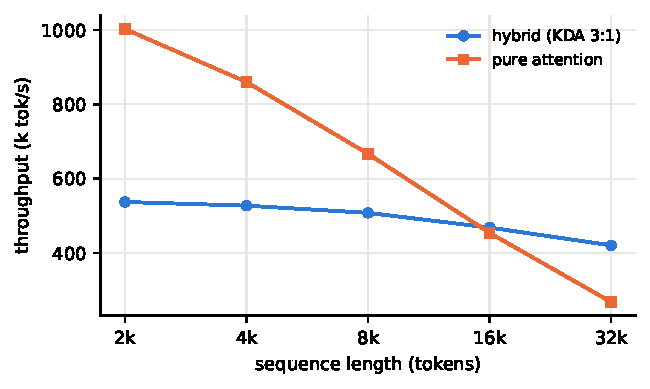
\includegraphics[width=0.62\textwidth]{figures/seq_sweep.pdf}
\caption{Throughput vs.\ sequence length, hybrid (3:1 KDA) against a
pure-attention control of the same size (TPU v6e-8). The recurrent
layers' linear scaling overtakes quadratic attention near 16k tokens;
at 32k the hybrid is $1.6\times$ faster. At the campaign's 2048 the
hybrid pays $\sim$2$\times$ for its richer mixer --- the price of buying
long-context headroom at training time.}
\label{fig:seqsweep}
\end{figure}

\section{Numerics and the precision policy}
\label{sec:numerics}

TPU matrix units evaluate an ``fp32'' matmul as one, three, or six
decomposed bf16 passes. The kernel's policy, called
\texttt{guarded\_fp32}, spends the passes exactly where the algebra is
fragile and nowhere else:

\begin{table}[h]
\centering
\small
\caption{Per-stage precision inside the fused kernels.}
\label{tab:precision}
\begin{tabular}{lll}
\toprule
stage & storage & matmul passes \\
\midrule
$q, k, v$ streams & bf16 & 1 \\
fast-weight state $S$, cumulative decay $G$ & fp32 & 1 \\
pairwise dots \eqref{eq:pairwise}, chunk scan & fp32 accum & 1 \\
WY inverse formation \eqref{eq:dc-inverse} & fp32 & 6 (v6e) / 3 emulated (v4) \\
inverse application, solve adjoints & fp32 & 6 (v6e) / 3 emulated (v4) \\
logits, softmax, loss & fp32 & --- \\
master weights, optimizer state & fp32 & --- \\
\bottomrule
\end{tabular}
\end{table}

Two measurements fix the policy's shape. First, running \emph{every}
stage at one pass is $4.9\times$ faster in the isolated core and
destroys the model: the loss reaches NaN by the second optimizer step.
Guarding only the solve recovers a stable loss curve at 561k tok/s ---
91\% of the full fused speedup. Second, the rejected repeated-squaring
solve (\S\ref{sec:inverse}) is a cautionary tale about validating on
real data: on random keys its intermediate powers stay tame, but
correlated real-text keys drive $\lVert T^{2^j} \rVert$ toward
$10^{12}$, and although the \emph{forward} answer survives, the backward
pass loses to catastrophic cancellation --- gradient norm 3{,}933.7
against a reference of 2.407. The divide-and-conquer inverse at three
emulated passes closes to a gradient norm of 2.406743 vs.\ the fp32
reference 2.406825 (relative $\ell_2$ error 1.86\% at cosine 0.99983),
and a per-layer sweep of solve condition numbers on checkpoint
activations ($\kappa_2 \le 10.4$, solve error $\le 2.3\times10^{-5}$
against fp64) qualified the 3-pass setting for the campaign.

The v4 3-pass mode is emulated in-kernel: each fp32 operand splits into
a bf16 high part and a bf16 residual, the three significant cross
products accumulate in fp32, and the dropped low$\times$low term is
bounded near $2^{-16}$ relative --- with a one-line rollback to six
passes kept in the source. Stability is a necessary but not sufficient
claim: the policy's residual 1.86\% gradient error is \emph{monitored},
not assumed away, and the campaign's loss/gradient telemetry
(\S\ref{sec:pretraining}) is the ongoing evidence that it never mattered.

\section{Optimizer: orthogonalized updates with a logit guard}
\label{sec:optimizer}

The optimizer, called \emph{MuonClip} in the codebase, routes every
parameter by role: two-dimensional ``matrix-like'' parameters (the KDA
projections, GQA QKV and output, both SwiGLU matrices) receive
orthogonalized momentum updates; everything else (embeddings, the tied
logit head, norm scales, biases, depthwise conv filters, the gate's
per-head scalars) receives AdamW. Routing is fail-closed: a parameter
with no declared role, or a matrix parameter without declared
factorization axes, is a build error rather than a silent default.

\subsection{The matrix update}

For a matrix gradient $M$ (after global clipping and momentum
$\beta = 0.95$ with Nesterov), the update direction is the approximate
orthogonalization of $M$ by a Newton--Schulz iteration on the normalized
matrix $X_0 = M / (\lVert M \rVert_F + \varepsilon)$:
\begin{equation}
X_{n+1} \;=\; a X_n + \big(b\, A_n + c\, A_n^2\big) X_n,
\qquad A_n = X_n X_n^{\top},
\qquad (a, b, c) = (3.4445,\, -4.7750,\, 2.0315),
\label{eq:ns}
\end{equation}
run for five iterations. The polynomial's fixed coefficients push every
singular value of $X$ toward 1, so the update has near-uniform spectral
footprint --- the property that lets small models take unusually large
stable learning rates. The applied update is scaled for consistent
root-mean-square magnitude across shapes,
\begin{equation}
\Delta W \;=\; -\,\eta \cdot 0.2 \sqrt{\max(\mathrm{fan_{in}},
\mathrm{fan_{out}})} \cdot \mathrm{NS}_5(M),
\label{eq:consistent-rms}
\end{equation}
which corrects a $6$--$10\times$ effective learning-rate undershoot that
the default width-scaling rule produces at these shapes. Scanned cycles
treat the scan axis as a batch of independent orthogonalization
problems; decoupled weight decay ($\lambda = 0.1$) and the learning-rate
schedule are shared with the AdamW arm
($\beta_1 = 0.9$, $\beta_2 = 0.95$, nesterov), and global gradient
clipping to norm 1 runs before either arm in fp32.

\subsection{QK-Clip for grouped-query attention}

Orthogonalized updates are known to permit slow unbounded growth of
attention logits over very long runs. As insurance, after each update
the fused QKV kernel of every cycle's attention layer is rescaled
whenever any head's maximum pre-softmax logit $s^{\max}_{c,h}$ (recorded
on-device across the global batch) exceeds a threshold $\tau = 100$:
\begin{equation}
\gamma_{c,h} = \min\!\left(1,\; \frac{\tau}{s^{\max}_{c,h} + \epsilon}\right),
\qquad
W_q^{(h)} \mathrel{*}= \sqrt{\gamma_{c,h}},
\qquad
W_k^{(j)} \mathrel{*}= \sqrt{\min_{h \in \mathrm{group}(j)} \gamma_{c,h}} .
\label{eq:qkclip}
\end{equation}
The grouped-query structure requires the adaptation on the right: a KV
head shared by several query heads takes the group's most conservative
scale, so the product of applied factors never exceeds any member
head's $\gamma$. Values and optimizer state are untouched.

The guard's cost--benefit is now measurable: across all 700{,}000
campaign steps the recorded maximum attention logit peaked at
\textbf{27.5} --- a factor 3.6 below the threshold. The clip never
fired. It cost one reduction and one conditional rescale per step and
bought the certainty that the run could not be lost to logit blow-up;
insurance that never paid out, priced at approximately zero.

\subsection{Learning-rate schedule}

The campaign schedule is warmup--constant--anneal:
\begin{equation}
\eta(t) =
\begin{cases}
\eta_{\max}\, t / t_w & t < t_w \quad \text{(brief linear warmup)}\\[2pt]
\eta_{\max} & t_w \le t < T - T_a \\[2pt]
\eta_{\max} \cdot \tfrac{1}{2}\big(1 + \cos \pi \tfrac{t - (T - T_a)}{T_a}\big)
& t \ge T - T_a,
\end{cases}
\label{eq:schedule}
\end{equation}
with $\eta_{\max} = 2 \times 10^{-3}$, total steps $T = 700\mathrm{k}$
and a terminal anneal of $T_a = 70\mathrm{k}$ steps. The constant
plateau keeps the option of extending the run open until the end; the
entire convergence benefit of decay is then collected in the final 10\%
of the budget (\S\ref{sec:pretraining}). The peak value itself came out
of an earlier sweep on the predecessor campaign, which found the
then-current setting roughly $10\times$ under-tuned --- with
consistent-RMS scaling \eqref{eq:consistent-rms}, $2\times10^{-3}$ is
comfortably stable for a 308M model.

\section{The yx49k tokenizer: an exact subset of the teacher}
\label{sec:tokenizer}

Most small models inherit a large general-purpose tokenizer and spend a
third or more of their parameters on the embedding table. We built a
49{,}152-token BPE with one additional structural requirement chosen for
what comes after pretraining: \emph{every} student token must correspond
to a distinct token of the Qwen3.5 vocabulary (the tokenizer of the 4B
model later used as a distillation teacher).

Formally, with student vocabulary $V_s$ ($|V_s| = 49{,}152$) and teacher
vocabulary $V_t$ ($|V_t| = 248{,}077$), the construction fixes an
injective map
\begin{equation}
m : V_s \hookrightarrow V_t
\qquad \text{such that } \mathrm{bytes}(i) = \mathrm{bytes}(m(i))
\;\; \forall i \in V_s,
\label{eq:subset-map}
\end{equation}
i.e.\ the student vocabulary \emph{is} a 49k-token sub-vocabulary of the
teacher's, selected by BPE training on a 545 MB multi-domain corpus
restricted to the teacher's token inventory (with a closure pass adding
8{,}366 tokens so every merge's constituents are present). The map has
two consequences measured at build time:
\begin{itemize}
  \item \textbf{Mass coverage.} On held-out teacher-domain text, the
  teacher assigns on average $98.75\%$ of its next-token probability
  mass to tokens in the image $m(V_s)$ (5th percentile $95.7\%$). The
  teacher's distribution restricted and renormalized to the student
  vocabulary is therefore a faithful target (\S\ref{sec:posttraining}).
  \item \textbf{Position alignment.} Any student-tokenized sequence maps
  token-by-token to a valid teacher input $m(x_1), \ldots, m(x_n)$ of
  the \emph{same length}, so teacher position $i$ scores exactly student
  position $i$. Distillation needs no edit-distance or byte-offset
  alignment machinery at all --- the failure class where student and
  teacher segmentations drift apart is impossible by construction.
\end{itemize}

Efficiency was not sacrificed. Held-out fertility is 1.0113
tokens/word-piece target, with 98.8\% of positions tokenized identically
to the teacher; on 1{,}041 ClimbMix documents the tokenizer achieves
4.637 characters per token --- within 3.2\% of a reference 128k-vocab
tokenizer at $2.6\times$ smaller vocabulary, and at parity with GPT-2's
50k. The 41-check build-time validation suite (round-trips, specials,
injectivity, coverage) passed in full.

\begin{table}[h]
\centering
\small
\caption{yx49k at a glance.}
\label{tab:tokenizer}
\begin{tabular}{ll}
\toprule
vocabulary & 49{,}152 (divisible by 128 through 4096) \\
construction & BPE over teacher-token inventory; injective $m: V_s \to V_t$ \\
teacher & Qwen3.5 (248{,}077 real tokens; 248{,}320 padded logit width) \\
teacher mass in-image & 98.75\% mean, 95.7\% p5 \\
held-out fertility & 1.0113; identical-to-teacher positions 98.8\% \\
compression & 4.637 chars/token on ClimbMix ($-3.2\%$ vs.\ 128k reference) \\
specials & 33 chat/tool tokens at ids 49119--49151 \\
embedding cost at $d{=}1024$ & 50.3M parameters \\
\bottomrule
\end{tabular}
\end{table}

Two variants ship: the canonical tokenizer (EOS \texttt{<|im\_end|>})
and a pretraining variant binding EOS to \texttt{<|endoftext|>}, keeping
the chat terminator out of the base distribution until the SFT stage.

\section{The pretraining campaign}
\label{sec:pretraining}

\subsection{Setup}

The model was trained on ClimbMix, a 400B-token filtered web corpus,
streamed and tokenized on the fly with a 50k-document shuffle buffer and
a 1\% held-out validation split. Hardware was a TPU v4-64 slice --- 32
chips across 8 hosts --- in pure data parallelism: per-device batch 8 at
sequence length 2048 gives
\begin{equation}
32 \times 8 \times 2048 = 524{,}288 \text{ tokens per optimizer step},
\end{equation}
and the 700{,}000-step budget totals $3.67\times10^{11}$ \emph{step
tokens}. Because the data stream restarts on resume (and the resumed
leg re-streams from a fresh shuffle), unique-token exposure is
$\sim$341B --- the final 26B of step tokens revisit the corpus head.
Throughput held at a median of 1.092M tokens/s (480 ms/step,
Fig.~\ref{fig:throughput}); against the v4 chip's nominal bf16 peak
this is a parameter-FLOP utilization of
\begin{equation}
\frac{6 \, N \, R}{32 \cdot 275\,\mathrm{TF}}
= \frac{6 \cdot 3.077\times10^{8} \cdot 1.092\times10^{6}}
       {8.8\times10^{15}} \approx 23\%,
\end{equation}
a lower bound that ignores all sequence-mixing FLOPs. Holdout loss was
evaluated every 2{,}500 steps and a ten-task lm-eval round ran on-device
every $\sim$20k steps, giving the campaign a benchmark trajectory, not
just an endpoint (Fig.~\ref{fig:evaltraj}).

\begin{figure}[t]
\centering
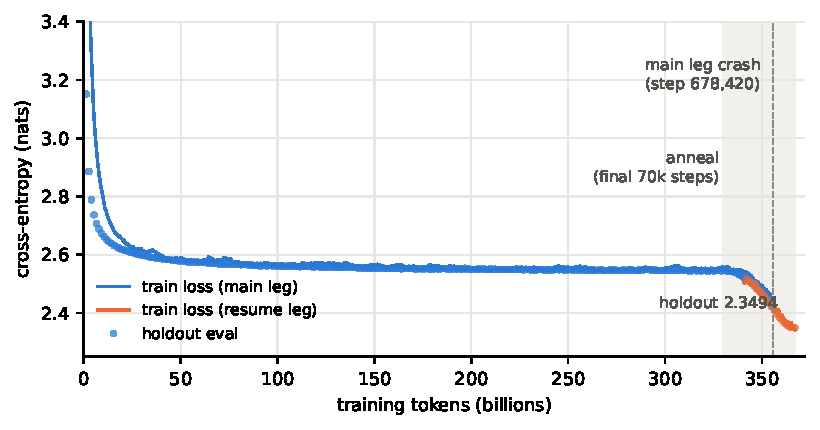
\includegraphics[width=\textwidth]{figures/pretrain_loss.pdf}
\caption{The campaign in one curve: train loss (smoothed) and holdout
evaluations for both W\&B legs against total training tokens. The
shaded band is the terminal anneal; the dashed line marks the main
leg's crash at step 678{,}420. The resume leg (orange) retraces the
main leg's trajectory through the overlap region before extending it
to 367B tokens and holdout 2.3494.}
\label{fig:loss}
\end{figure}

\subsection{Schedule and anneal}

The learning rate followed \eqref{eq:schedule}: brief warmup, then a
constant $2\times10^{-3}$ for 90\% of the run, then cosine to zero over
the final 70k steps (Fig.~\ref{fig:lr}). The anneal is where the
campaign cashed in: holdout fell from 2.5446 (step 620k, pre-anneal) to
2.3494 --- $-0.195$ nats, roughly the same improvement as the preceding
300k constant-rate steps combined --- and every benchmark in the
trajectory bent visibly upward through the shaded region of
Fig.~\ref{fig:evaltraj} (HellaSwag $49.3 \to 56.9$, Lambada
$40.4 \to 47.4$ over the final 80k steps). The benchmark curve was still
rising at step 700k; the budget, not convergence, ended the run.

\begin{figure}[t]
\centering
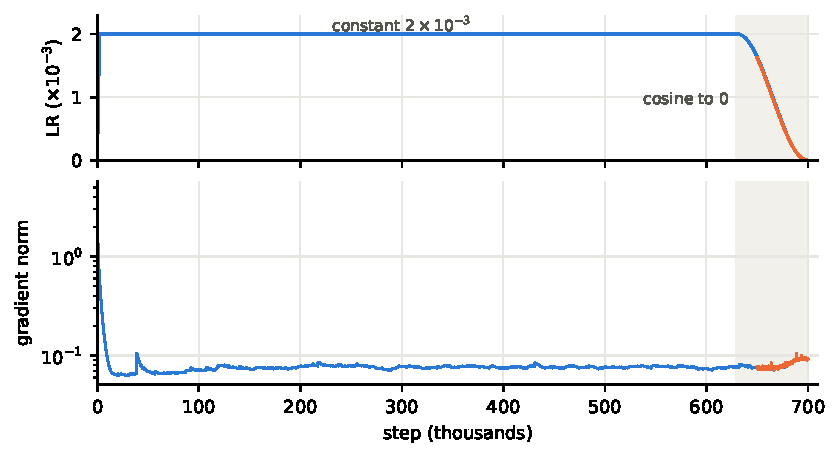
\includegraphics[width=\textwidth]{figures/lr_gradnorm.pdf}
\caption{Learning-rate schedule (top) and smoothed gradient norm
(bottom, log scale) across both legs. The resume leg's schedule
overlays the main leg's exactly through the overlap --- the optimizer
restored to the same trajectory. The gradient norm is flat at
$\sim$0.07 for the entire constant-rate phase; no clipping events, no
spikes, no drift.}
\label{fig:lr}
\end{figure}

\begin{figure}[t]
\centering
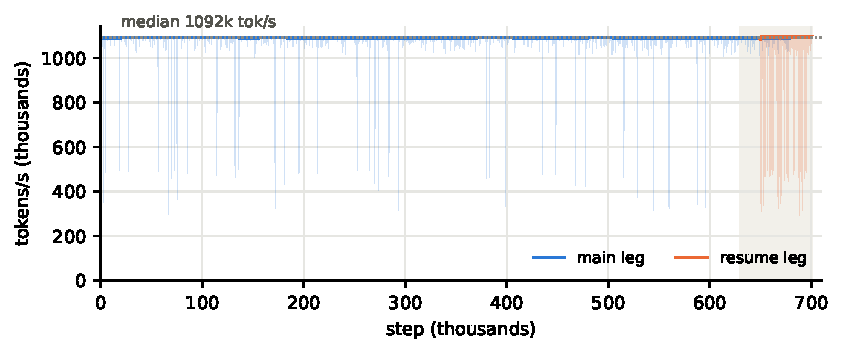
\includegraphics[width=\textwidth]{figures/throughput.pdf}
\caption{Slice throughput over the campaign (rolling median over raw
per-step rates; faint traces show the raw series, whose dips are eval
and checkpoint pauses). The line is flat at 1.09M tokens/s for four
days of wall time --- the data pipeline, running host-side over
streamed HF shards, never became the bottleneck.}
\label{fig:throughput}
\end{figure}

\subsection{The crash, and what a clean resume looks like}

At step 678{,}420 --- 22k steps from the finish, inside the anneal ---
the main leg died (W\&B state \emph{crashed}; the slice itself
survived). Training resumed three days later from the most recent
durable checkpoint ($\approx$ step 650k) as a second W\&B leg,
re-running steps 650k--700k with a restarted data stream.

The resume's fidelity is measurable rather than assumed, three ways.
First, the loss curves: through the 28k-step overlap the resumed leg
retraces the original to within smoothing width (Fig.~\ref{fig:loss}).
Second, the schedule: the resumed learning-rate curve lands exactly on
the original cosine (Fig.~\ref{fig:lr}). Third, the benchmark round at
step 660k, which both legs executed, agreed within noise (HellaSwag
$51.9$ vs.\ $51.3$, ARC-e $63.0$ vs.\ $62.7$) despite the different
shuffle --- the model state, not the data order, determines the
trajectory at this point in training. The campaign's conclusion is
thereby independent of the crash: the final 700k-step model is the same
model the uninterrupted run would have produced, up to data-order noise
that the 660k A/B bounds at a few tenths of a point.

\begin{figure}[t]
\centering
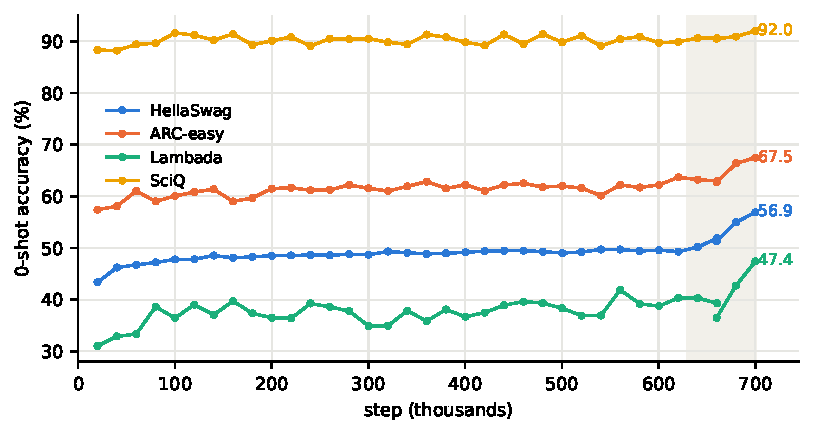
\includegraphics[width=\textwidth]{figures/eval_trajectory.pdf}
\caption{In-training 0-shot benchmark trajectory (both legs), one
lm-eval round per $\sim$20k steps. Long plateaus through the
constant-rate phase, then the anneal (shaded) lifts every task
simultaneously --- the argument, in one figure, for spending the last
10\% of any fixed budget on a terminal anneal.}
\label{fig:evaltraj}
\end{figure}

\section{Base-model evaluation}
\label{sec:evaluation}

All numbers below are 0-shot lm-eval results for the step-700k
checkpoint unless marked otherwise; reference models are quoted at their
published settings.

\begin{table}[h]
\centering
\small
\caption{0-shot suite at step 700k, against same-class references.
``prev gen'' is this project's predecessor campaign (337M, 40B
tokens, 128k-vocab tokenizer).}
\label{tab:evals}
\begin{tabular}{lcccccc}
\toprule
task & \textbf{ours} & SmolLM2 & SmolLM & Qwen2.5 & Gemma3 PT & prev gen \\
 & 308M / 0.37T & 360M / 4T & 360M / 0.6T & 0.5B & 270M & 337M / 40B \\
\midrule
HellaSwag & \textbf{56.9} & 54.5 & 51.8 & 51.2 & 40.9 & 50.6 \\
ARC avg & \textbf{53.8} & 53.0 & 50.1 & 45.4 & 43.4 & 48.9 \\
PIQA & \textbf{75.2} & 71.7 & 71.6 & 69.9 & 67.7 & 72.1 \\
OpenBookQA & \textbf{38.8} & 37.4 & 37.2 & 37.4 & --- & 36.2 \\
BoolQ & 58.0 & --- & --- & --- & 61.4 & 60.1 \\
\midrule
Lambada & 47.4 & \multicolumn{5}{l}{SciQ 92.0 \quad COPA 72.0 \quad
ARC-e/c 67.5 / 40.1} \\
\bottomrule
\end{tabular}
\end{table}

\begin{figure}[t]
\centering
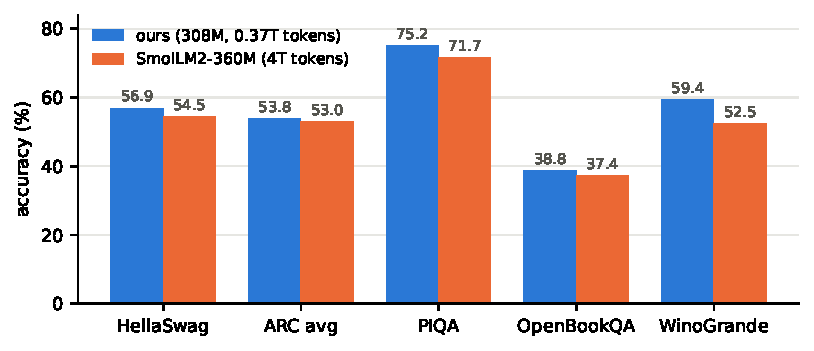
\includegraphics[width=0.9\textwidth]{figures/eval_bars.pdf}
\caption{Ours vs.\ the strongest same-size reference. The model is
ahead on every comparable row while having seen $\sim$1/11 the
pretraining tokens.}
\label{fig:evalbars}
\end{figure}

The headline is the data efficiency: the model beats SmolLM2-360M ---
the strongest same-size open reference, trained on 4T tokens --- on
every row where the numbers are comparable, from an 11$\times$ smaller
token budget. Three further panels complete the picture:

\begin{table}[h]
\centering
\small
\caption{Post-hoc loglikelihood and generation panels (step 700k).}
\label{tab:panels}
\begin{tabular}{llll}
\toprule
task & ours & best same-class reference & note \\
\midrule
WinoGrande 0-shot & \textbf{59.4} & SmolLM-360M 52.8 & $+5$ over every reference \\
WinoGrande 5-shot & \textbf{57.9} & Qwen2.5-0.5B 54.1 & \\
MMLU cloze 0-shot & 30.0 & SmolLM2-360M 35.8 & between SmolLM 135M/360M tiers \\
TriviaQA 5-shot & 15.3 & SmolLM2-360M 16.9 & parity with Gemma3 PT (15.4) \\
GSM8K 5-shot & 1.1 & SmolLM2-360M 3.2 & base-model band, pre-SFT \\
\bottomrule
\end{tabular}
\end{table}

WinoGrande is the standout --- $+5$ points over every reference on a
task where this size class barely clears chance --- and, with HellaSwag
and PIQA, suggests the architecture's strength is concentrated in
commonsense/coreference resolution. The two knowledge-bound scores
(MMLU cloze, TriviaQA) track factual \emph{exposure} rather than
capability and sit where an 0.37T-token diet predicts: this is the axis
post-training distillation from a knowledge-rich teacher targets next.
CommonsenseQA in standard format scores 26.2; small base models cluster
at chance there, and published references using cloze formulations are
not comparable.

\section{Post-training: SFT and offline logit distillation}
\label{sec:posttraining}

Post-training proceeded in two stages: supervised fine-tuning to install
the chat format, then offline logit distillation from a frozen
Qwen3.5-4B teacher to install the teacher's token-level distribution.
Every stage decision below was fixed by a measured A/B rather than
convention; the ledger records nulls as prominently as wins.

\subsection{Data}

SFT used the Mephisto instruction corpora together with a large public
SFT mix (6.27M rows total, minimum packing length 4096). Two of the
Mephisto sets --- \texttt{Mephisto-IF\_172k} (instruction following) and
\texttt{Mephisto-Knowledge\_538k} (knowledge), published under the
\texttt{Yxanul} organization --- were generated on a TPU \emph{v6e}
slice with this project's own batched decoding stack;
\texttt{Mephisto-MathCode\_2M} completes the mix with third-party
math/code completions. The distillation stage draws prompts from the
same pools but replaces the completions' one-hot supervision with
teacher distributions.

\subsection{The distillation objective}

\paragraph{Teacher projection.} The subset map \eqref{eq:subset-map}
makes the teacher's distribution directly comparable to the student's.
Given teacher logits $z^{T} \in \R^{|V_t|}$ at a position (truncated to
the 248{,}077 real rows of the padded 248{,}320-wide head --- padded
embedding rows emit real logits and must be excluded), the projected
teacher log-probabilities on the student support and the residual mass
are
\begin{equation}
\ell_i = z^{T}_{m(i)} - \log\!\!\sum_{v \in V_t}\!\! e^{z^{T}_v}
\quad (i \in V_s),
\qquad
\rho = 1 - \sum_{i \in V_s} e^{\ell_i},
\label{eq:projection}
\end{equation}
computed with a blockwise log-sum-exp (block 32{,}768, per-block fp32
cast). The residual $\rho$ --- the teacher's mass outside the student's
image, $\sim$1.25\% on the training mixture per
\S\ref{sec:tokenizer} --- is \emph{reported and renormalized away},
never trained against. Because $m$ is injective and length-preserving,
teacher position $i$ supervises student position $i$ with no alignment
pass; the property was verified empirically by checking that shifting
the teacher by one position strictly worsens agreement.

\paragraph{Divergence.} With renormalized teacher
$p_i = e^{\ell_i}/(1-\rho)$ and student $q = \mathrm{softmax}(z^{S})$,
the general objective is a $\beta$-weighted Jensen--Shannon divergence,
\begin{equation}
D_\beta(p \,\|\, q) \;=\; \beta \KL{p}{m_\beta} + (1-\beta)\KL{q}{m_\beta},
\qquad m_\beta = \beta p + (1-\beta) q,
\label{eq:jsd}
\end{equation}
with the convention that $\beta$ weights the \emph{teacher}, so
$\beta \to 0$ recovers forward KL $\KL{p}{q}$ (mass-covering) and
$\beta \to 1$ reverse KL (mode-seeking); the small-$\beta$ limit
$D_\beta \approx \beta \KL{p}{q}$ is pinned by a unit test, guarding the
orientation. The campaign ran $\beta = 0$ throughout.

\paragraph{Top-$K$ compression and the coverage term.} Storing full
49k-wide teacher distributions is wasteful; the pipeline precomputes,
once per example, the teacher's top-$K$ ($K \in \{32, 64\}$,
$\sim$90 bytes/position at $K{=}32$ compressed) via an approximate
top-$K$ (recall 0.95; exact top-$k$ lowers to a full sort on TPU and is
$87\times$ slower --- a missed boundary entry simply stays in the tail
bucket). With kept set $\mathcal{K}$, tail $r = 1 - \sum_{i \in
\mathcal{K}} e^{\ell_i}$, and renormalized teacher $\tilde{p}$ on
$\mathcal{K}$, the $\beta{=}0$ loss uses the student's \emph{raw}
probabilities at the kept ids:
\begin{equation}
D \;=\; \sum_{i \in \mathcal{K}} \tilde{p}_i
\big(\log \tilde{p}_i - \log q_i\big)
\;=\;
\underbrace{\KL{\tilde{p}}{\tilde{q}}}_{\text{truncated forward KL}}
\;\; \underbrace{- \log\!\!\sum_{i \in \mathcal{K}}\!\! q_i}_{\text{coverage}},
\label{eq:topk}
\end{equation}
where $\tilde{q}$ is the student renormalized on $\mathcal{K}$. The
decomposition on the right is the design: an exact truncated forward KL
plus a penalty on student mass leaking outside the teacher's top-$K$
--- non-negative, and zero exactly when the student matches the
renormalized teacher on $\mathcal{K}$ and carries no outside mass. At
$K = |V_s|$ the compression is exact and \eqref{eq:topk} reproduces the
full-support loss (also pinned by test). The composite objective
$\mathcal{L} = w_d D + w_{ce}\,\mathrm{CE}$ shares one masked-position
denominator between both terms; the campaign ran pure distillation
($w_d = 1$, $w_{ce} = 0$) with CE logged as a monitor.

\begin{figure}[t]
\centering
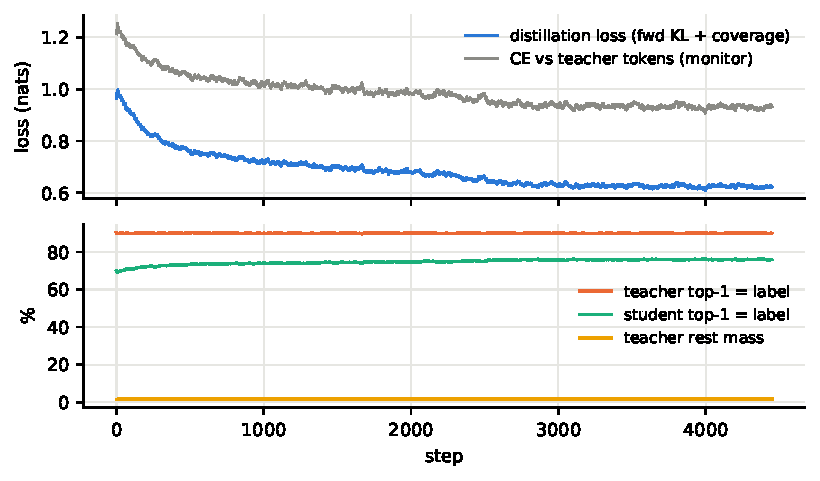
\includegraphics[width=\textwidth]{figures/gold_curves.pdf}
\caption{The 300k-example distillation run (top: losses; bottom:
top-1 agreement and residual mass). The distillation loss falls 37\%
while the CE monitor barely moves --- the student is learning the
teacher's \emph{distribution}, not memorizing tokens. Teacher top-1
agreement with the data's labels sits at 90\% (an upper reference),
student agreement climbs toward 76\%, and the teacher's rest mass
holds near 1.5\%.}
\label{fig:gold}
\end{figure}

\subsection{Results ladder and the epoch null}

\begin{table}[h]
\centering
\small
\caption{The post-training lineage. IFEval is the mean of the four
strict/loose prompt/instruction accuracies; panel is a 42-prompt scored
transcript battery. All decoding at each checkpoint's swept settings.}
\label{tab:lineage}
\begin{tabular}{llcc}
\toprule
checkpoint & recipe & IFEval & panel /42 \\
\midrule
gen-2 & base + SFT 690k rows & 40.4 & 10 \\
GOLD-10k & gen-2 + distill 10k IF & 42.1 & --- \\
GOLD-50k & gen-2 + distill 50k IF & 48.4 & 12 \\
GOLD-mix300k & gen-2 + distill 100k$\times$\{IF, Know, MathCode\} & \textbf{51.0} & 16 \\
SFT-6M & base + SFT 6.27M rows & 35.3 & 15 \\
GOLD-over-SFT & SFT-6M + distill 1/3 mix, $K{=}32$ & 41.3 & \textbf{22} \\
\;(2-epoch control) & same store, 2 epochs & 40.3 & 22 \\
\bottomrule
\end{tabular}
\end{table}

Three findings organize the ladder. \emph{Distillation dominates SFT
per row}: 300k distilled examples beat 6.27M one-hot rows by $+15.7$
IFEval --- soft targets carry more supervision per example than hard
labels by more than an order of magnitude at this scale. \emph{Mixed
diets beat matched diets}: distilling knowledge and math/code rows
alongside instruction data improved \emph{instruction following} beyond
what pure-IF distillation achieved. \emph{One epoch per store}: a
controlled second epoch over the same precomputed targets moved the
training loss ($0.504 \to 0.480$) and nothing downstream (IFEval
$41.3 \to 40.3$, panel $22 \to 22$) --- the marginal unit of compute
belongs to fresh rows, not repetition.

\section{External calibration}
\label{sec:calibration}

Published numbers do not transfer across evaluation harnesses, so the
final calibration measured every model under this project's own
conventions: identical prompts, identical scoring code, IFEval with the
same chat-template and generation settings, and each model decoded at
its documented or swept-best settings. The references are the three
strongest openly available instruction-tuned models near 300M:
Gemma~3 270M IT, SmolLM2-360M-Instruct, and SmolLM-360M-Instruct.

\begin{table}[h]
\centering
\small
\caption{Everything measured, one harness. Panel: 42 scored prompts
(knowledge/math/code/instruction-format). Chat: 12 freeform prompts with
lenient checkers. Loglik: measured 0-shot (hellaswag / arc-c / piqa /
winogrande). IFEval: mean of the four accuracies.}
\label{tab:calibration}
\begin{tabular}{lcccc}
\toprule
 & SmolLM-IT & Gemma3 IT & \textbf{ours} & SmolLM2-IT \\
 & 360M / 0.6T & 270M / 6T & 308M / 0.37T & 360M / 4T \\
\midrule
panel /42 & 19 & 31 & 22 & \textbf{34} \\
chat /12 & 10 & 8 & 9 & \textbf{11} \\
IFEval (GOLD-over-SFT / mix300k) & 16.1 & 31.4 & 41.3 / \textbf{51.0} & 40.1 \\
loglik: hellaswag & 52.7 & 37.7$^{\dagger}$ & 53.5 & \textbf{56.8} \\
loglik: arc-challenge & 33.0 & 28.2$^{\dagger}$ & \textbf{37.5} & 34.0 \\
loglik: piqa & 70.6 & 66.2$^{\dagger}$ & \textbf{73.4} & 71.3 \\
loglik: winogrande & 53.6 & 52.3$^{\dagger}$ & \textbf{58.0} & 57.6 \\
\bottomrule
\multicolumn{5}{l}{\footnotesize $^{\dagger}$Gemma's published IT numbers
(0-shot, matching tasks); its measured IFEval of 31.4 sits far below its}\\
\multicolumn{5}{l}{\footnotesize published 51.2 --- the concrete case for
measuring everything under one harness.}
\end{tabular}
\end{table}

The matrix separates two axes cleanly. On \emph{capability} (the
loglikelihood rows) our model leads 3/4 against every reference, from
11--16$\times$ less pretraining data; only SmolLM2's 4T tokens buy it
one row (HellaSwag). On \emph{behavior} (the transcript panel) the
deeply post-trained references lead: SmolLM2's mature SFT+preference
pipeline yields drilled math/code answer rituals (8/8 and 8/8 on those
panel sections vs.\ our 4/8, 4/8) and disciplined termination, while our
transcripts' signature failure is producing the \emph{correct} answer
and then destroying it in continued generation --- computing 144 and
talking itself to 1440, repeating a birthday greeting thirty-six times.
Notably, our IFEval still leads all references (mix300k's 51.0 is
$+10.9$ over the best measured reference), and the same-family
SmolLM v1$\to$v2 jump (panel $19 \to 34$, IFEval $16.1 \to 40.1$ at
identical parameter count) is an existence proof that everything
separating the columns is data and post-training recipe --- not
architecture, and not size.

The failure signature also names the cure. Right-answer-then-drift is
textbook exposure bias: teacher-forced training (SFT and offline
distillation alike) never shows the model its own repetition spirals, so
nothing ever penalizes them. On-policy distillation --- sampling from
the student and letting the teacher score the student's own
continuations --- attacks exactly this, and is the designated next stage.

\section{Discussion and future work}
\label{sec:discussion}

\paragraph{What the evidence supports.} At the 300M scale, this program
found (i) architecture and data quality dominate raw token count --- a
0.37T-token hybrid beats a same-size 4T-token reference on most
capability measures; (ii) the terminal anneal is the highest-leverage
10\% of a fixed pretraining budget; (iii) soft-target distillation
carries over an order of magnitude more supervision per example than
one-hot SFT; and (iv) the remaining gap to the best same-size
instruction models is decode-time discipline --- a post-training
property, purchasable at this size, as the SmolLM v1$\to$v2 delta
demonstrates.

\paragraph{Limitations.} The base model's knowledge-bound axis (MMLU,
TriviaQA) reflects its token budget and remains below the 4T-token
reference. Strict-format instruction following is hard for every model
measured at this size; the best reference reaches 5/8 on that panel
section where we reach 3/8. The repetition spiral survives offline
distillation; whether it survives on-policy training is the next
experiment's question, and the honest possibility remains that some of
it is a capacity effect. All pretraining ran at sequence length 2048;
the architecture's long-context economics
(Fig.~\ref{fig:seqsweep}) are demonstrated for throughput but not yet
exercised by training.

\paragraph{Next.} In order of expected value: an on-policy distillation
stage (student-sampled rollouts scored by the teacher --- directly
targeted at the observed failure class); the full offline campaign over
the remaining prompt pools at $K{=}32$ with termination-weighted data;
and a width/depth scale-up for which the measured groundwork (an 884M
configuration's loss-head and sharding sweeps) already exists in the
repository. The comparison battery of \S\ref{sec:calibration} is fully
scripted and will be re-run unchanged after each stage; the bar it sets
is precise --- match SmolLM2-360M-Instruct's 34/42 transcript discipline
while keeping the capability and IFEval leads --- and clearing it would
make this the strongest model of its size class outright.

\paragraph{Acknowledgments.} Compute was provided by the TPU Research
Cloud. The pretraining corpus is ClimbMix; evaluation uses the
EleutherAI lm-evaluation-harness; the distillation teacher and the
tokenizer's parent vocabulary are Qwen3.5.


\part{A 1B Multimodal Program}

\section{A 1B multimodal architecture}
\label{sec:vision-arch}

Part II scales the Part I recipe to a $\sim$0.98B-parameter model and
adds native vision. The backbone keeps the depth-first hybrid cycle
\([\mathrm{KDA},\mathrm{KDA},\mathrm{KDA},\mathrm{GQA}]\) with
\(d_{\mathrm{model}}{=}1536\), 32 layers (8 cycles), SwiGLU MLPs of
width 4096, 12 KDA heads of dimension 128, GQA \(12{:}3\), and the
yx49k tied embedding. Two deliberate departures from Part I:

\paragraph{Standard residuals.} The depth-attention residual policy of
Part I moves a \([\,\text{depth},B,T,d\,]\) buffer through both scan
directions; at this width and sequence length 4096 that buffer costs a
measured 736\,ms of a 2{,}309\,ms step (its copies alone are half of
that). Plain pre-norm residuals recover $+47\%$ throughput, and with
two further measured levers (unfused MLP, parameter scan on axis 0)
the operating point reaches 342k tokens/s on 32 TPU\,v4 chips at
23.9\% parameter-FLOP utilization --- above the tuned Part~I campaign.

\paragraph{A head-specific sigmoid output gate.} Part I's campaign
telemetry recorded a permanent collapse of the first cycle's attention
logits (all heads pinned at exactly zero from step $\sim$35k onward).
Each GQA layer here therefore gates its per-head SDPA output
elementwise by \(\sigma(W_g x)\) \emph{before} the output projection,
with \(x\) the same normalized hidden state that feeds QKV. The bet is
validated in Section~\ref{sec:vision-campaigns}: cycle-0 heads remain
active through and far beyond the horizon at which the ungated model
collapsed.

\paragraph{The vision tower.} Vision is trained from scratch, jointly,
under the next-token objective alone --- no contrastive stage, no
pretrained encoder. A ViT-S-class tower (12 bidirectional pre-norm
blocks, width 384, 6 heads, MLP 1536; RMSNorm, bias-free) embeds
\(448^2\) images as \(28^2\) patches of size 16; a \(2{\times}2\)
space-to-depth fold and a two-layer projector map them to 196 visual
tokens in the language embedding space. Images enter the token stream
as runs of a reserved placeholder id whose embeddings are replaced by
the tower's output; the loss never lands on placeholder positions. The
tower's matrices join the Muon partition; its patch embedding and
learned 2D positions join the AdamW side, mirroring the Part~I routing
philosophy.

\paragraph{Packing.} Mixed batches pack whole rows (an image row: 196
placeholders + its dialogue; a text row: one truncated document) into
4096-token sequences with per-row segment ids and restarting
positions. Segment masking confines attention and loss to each row;
the KDA recurrent state is not reset at row boundaries --- it only
decays, with the per-token log-decay bounded by the safe gate, a
carryover the 50B-token Part~I SFT already tolerated and which two
campaigns here confirm benign.

\section{Streaming a measured multimodal mixture}
\label{sec:vision-data}

Both campaigns stream everything: no corpus is materialized on disk.
Each of the 8 hosts holds one producer thread whose sources are sharded
at the \emph{file} level (a row-modulo shard would download every
shard's rows and discard $7/8$ of them). The composition is controlled
where it matters --- in supervised (loss) tokens, not in rows --- and
every knob has a live instrument.

\paragraph{Composition by calibration.} A row-level Bernoulli chooses
vision versus text; a weighted draw chooses the text source. Row
weights are not the supervision mix: an image row contributes mostly
loss-free placeholder positions, and source documents differ in length.
Weights are therefore solved from a decomposed calibration --- measured
mean supervised tokens per row per source --- and verified against the
live per-source loss-token shares. The continuation's realized mix held
constant to three decimals across 57{,}220 steps:

\begin{center}
\begin{tabular}{lrr}
\toprule
source & target share & realized share \\
\midrule
vision dialogue (FineVision-class) & 0.35 & 0.359 \\
web text (ClimbMix) & 0.40 & 0.404 \\
source code (Stack-class, one file per row) & 0.17 & 0.158 \\
mathematics (CC-derived, quality-filtered) & 0.08 & 0.079 \\
\bottomrule
\end{tabular}
\end{center}

Code rows carry file \emph{content only} --- no paths or repository
metadata enter the token stream; the packer's per-row segments are the
file boundaries.

\paragraph{Budget-aware fill.} The first measured pathology was
packing waste: when a drawn image row exceeded a sequence's 4-image
budget, the packer ended the sequence early, and padding still costs
full compute --- a measured \(\mathrm{pad}=0.279\) at the initial
setting. Ending a pack now triggers a text-only fill of the remaining
capacity (stashed rows open later sequences; nothing is dropped or
duplicated), taking padding to \(0.04\)--\(0.06\).

\paragraph{Bytes are the bottleneck, twice.} Shipping image pixels as
fp32 cost 154\,MB per host per step, and the host-side global-array
assembly ran at a median 1{,}802\,ms against a 1{,}504\,ms device step
--- the dominant throughput loss of the first campaign (75.7\% of 8.3
wall-hours of excess). Pixels now travel as uint8 and normalize on
device (the same \(a/255\cdot2-1\) mapping, verified end-to-end
through the tower); assembly drops under the device window and the
sustained rate recovers to the 348k tokens/s floor.

\paragraph{Self-healing streams.} A multi-day streaming run loses HTTP
clients in varied ways --- hung reads, closed-client errors after retry
aborts, transient object-store failures --- and on a synchronous
8-host slice any one host's stall idles all 32 chips. Every stream
draw therefore reopens its stream with a fresh client on any
exception, with bounded backoff; a dead client costs one host seconds
instead of the fleet an hour. After this change the second campaign
ran 49{,}220 steps without a single stream incident.

\section{Two campaigns: 25B + 30B tokens}
\label{sec:vision-campaigns}

\begin{figure}[t]
\centering
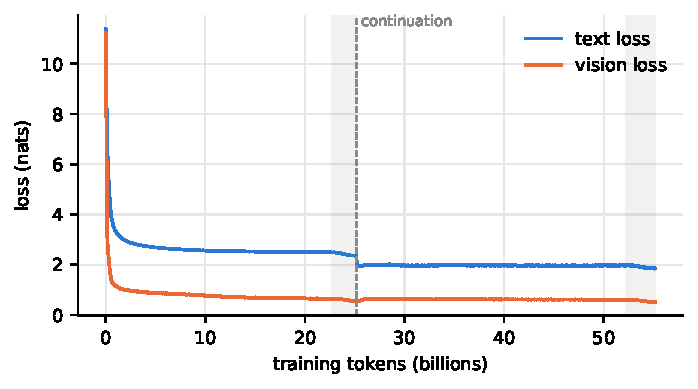
\includegraphics[width=0.94\linewidth]{figures/vision_loss_curves.pdf}
\caption{Vision and text loss across both campaigns on one cumulative
axis (EMA-smoothed). Shaded spans are the two terminal anneals; the
dashed line marks the warm-start into the continuation, whose re-warmed
learning rate briefly gives back the first anneal's polish.}
\label{fig:vision-loss}
\end{figure}

\textbf{Trial (48{,}000 steps, 25.2B tokens).} From-scratch joint
training at sequence length 4096, per-device batch 4 (524{,}288
tokens/step), MuonClip at LR $1.2\times10^{-3}$, terminal cosine anneal
over the final 4{,}800 steps. The tower's output scale told the run's
most instructive story (Figure~\ref{fig:embed-ratio}): unconstrained by
any output norm, the visual/text embedding RMS ratio overshot from 0.60
to 4.98 by step 5k, then declined monotonically as the loss pulled the
tower onto the language manifold --- no intervention required, which is
precisely what the probe was built to establish.

\begin{figure}[t]
\centering
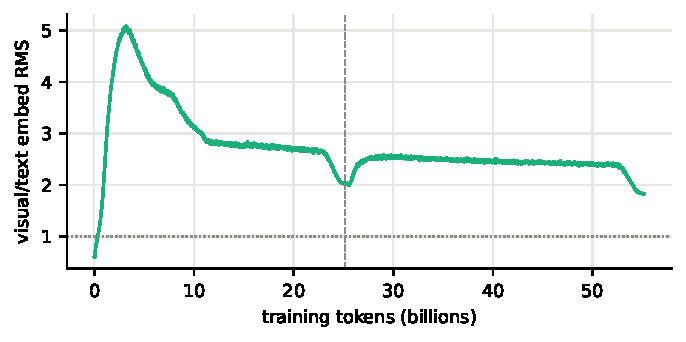
\includegraphics[width=0.94\linewidth]{figures/embed_ratio.pdf}
\caption{Post-splice visual/text embedding RMS ratio. The from-scratch
tower overshoots the language scale $5\times$ early, then
self-regulates; each anneal pulls it further toward parity.}
\label{fig:embed-ratio}
\end{figure}

\textbf{Continuation (57{,}220 steps, 30.0B tokens).} Warm-started from
the trial's annealed checkpoint with a fresh optimizer and a 1{,}500-step
re-warmup, adding the code and mathematics streams of
Section~\ref{sec:vision-data}. One observation deserves record: through
the continuation's terminal anneal the \emph{pure web-text} holdout
degraded by $\sim$0.1 nats while the training mixture kept improving
--- as the learning rate vanishes the model converges precisely to the
\emph{mixture} optimum, exposing its distance from the pure-text
optimum. Convergence reveals allocation; the capability sections show
what the reallocation bought.

\textbf{Stability.} Across 105{,}220 steps and 55B tokens: zero
non-finite losses or gradients, zero QK-clip activations, and --- the
gate's validation --- cycle-0 attention max-logits alive in the 8--14
band throughout, including the step-30k--40k window where Part~I's
ungated campaign collapsed permanently to zero. Gradient norms stayed
in the 0.04--0.14 band with the tower's share rising $15\times$ as
visual features became load-bearing.

\textbf{Operations.} Each campaign survived one mid-run failure
(a hung parquet read without a timeout; a closed HTTP client), both
recovered by weights-and-optimizer resume from 4{,}000-step per-host
local checkpoints with the stream restarting --- the streaming
checkpoint policy of Part~I unchanged. Both root causes were then
eliminated in code (timeouts; the self-healing draw), not in runbooks.

\section{What 55B multimodal tokens buy}
\label{sec:vision-results}

\begin{figure}[t]
\centering
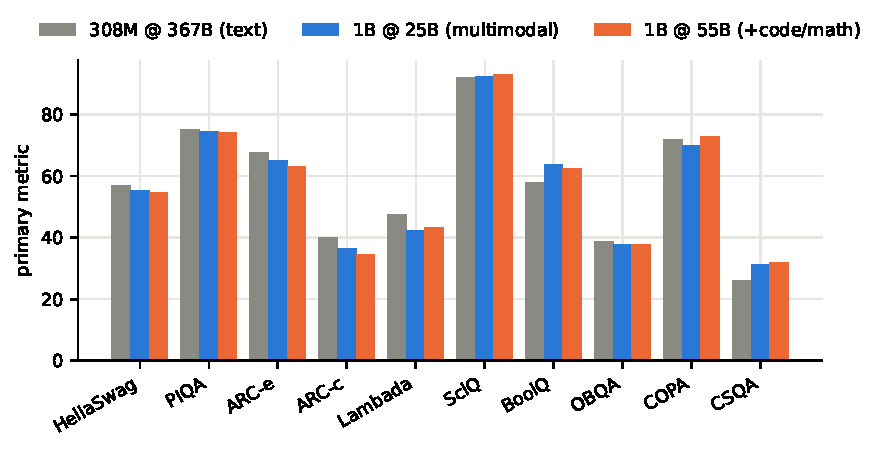
\includegraphics[width=\linewidth]{figures/vision_eval_bars.pdf}
\caption{Zero-shot primary metrics: the 308M text model at its full
367B-token budget versus the 1B multimodal model at 25B and 55B
tokens.}
\label{fig:vision-evals}
\end{figure}

\paragraph{Language holds at a fraction of the text budget.} With only
$\sim$12.8B of its supervised tokens on web text, the 25B-token trial
already beats the 337M 50B-token baseline of Part~I on every anchor,
and sits within a few points of the full 367B-token 308M campaign on
most (Figure~\ref{fig:vision-evals}); it is ahead outright on BoolQ
($+5.7$) and CommonsenseQA ($+5.2$). The continuation's added code and
mathematics leave this profile flat --- by design, its budget went
elsewhere: GSM8K (5-shot, full test set, greedy through the
incremental decoder) rises from 1.21\% to \textbf{3.18\%} exact-match,
versus 1.1\% for the 308M model at $6.7\times$ the text tokens.

\paragraph{Vision is grounded, not memorized.} On held-out probes the
final model counts objects, discriminates left from right, reads
synthetic and document text, identifies chart structure with values
read to within half a point, and localizes UI elements on screenshots
from shards the training pass never reached (a requested click lands
within 0.2\% in $x$). The trial model failed counting, mirrored
left/right, and refused synthetic OCR; thirty billion further tokens
repaired all three --- the classic small-VLM failure modes are budget
artifacts, not architectural ones.

\paragraph{Post-training transfers unchanged.} Because the 1B shares
Part~I's tokenizer, the entire post-training stack --- chat SFT and
GOLD distillation, including the \emph{same precomputed teacher
stores} --- applies verbatim. One day sufficed for four checkpoints:

\begin{center}
\begin{tabular}{lccc}
\toprule
checkpoint & IFEval mean & panel (32) & clean stops \\
\midrule
SFT-1 (dialogue-only mix) & 35.0 & 12 & 0/32 \\
\; + GOLD & 40.8 & 24 & 31/32 \\
SFT-2 (instruction-dense mix) & \textbf{55.3} & 23 & 32/32 \\
\; + GOLD & 48.8 & \textbf{27} & 32/32 \\
\midrule
308M best (Part I, GOLD) & 51.0 & --- & --- \\
\bottomrule
\end{tabular}
\end{center}

The instruction-dense second mix at a bolder learning rate is worth
$+20.3$ IFEval points over the first --- past every Part~I checkpoint
--- and distillation on top trades 6.5 of those points for the best
answer quality of the project (27/32), the teacher's discursive style
partially overwriting strict-format obedience. Constraint-following
tracks instruction-dense exposure; answer quality tracks the teacher:
the two live on a measurable frontier, and both frontier points belong
to the 1B.

\paragraph{Limitations.} GSM8K remains near-floor in absolute terms;
fine-grained visual categories and blocky synthetic text remain
brittle; instruction obedience at the strictest level trails what 367B
text tokens buy. Each gap moved monotonically with tokens in these
two campaigns, which is the scaling argument in its plainest form.


\appendix
\section{Kernel experiment ledger (digest)}
\label{app:ledger}

The kernel program ran as 42 numbered experiments over nine days on a
TPU v6e-8, then a v4-64. The decision path, compressed:

\begin{table}[H]
\centering
\small
\begin{tabular}{lp{11cm}}
\toprule
EXP-001..008 & Baselines: 272M dense transformer, INT8 rejected,
modern GQA recipe, orthogonalized-momentum optimizer adopted. \\
EXP-009..015 & KDA implemented (reference recurrence, chunkwise form);
3:1 hybrid matched for throughput; external kernel codebases audited
--- only the state-scan skeleton proved reusable. \\
EXP-016..023 & The backward problem: blocked Pallas solve, analytical
XLA VJP (31.9 ms), then the fused Pallas pair (18.3 ms core); grid
collapse and selective bf16 (\S\ref{sec:numerics}) reach 616k tok/s
full-model. \\
EXP-024..028 & Batch/remat/sequence sweeps; the 16k crossover of
Fig.~\ref{fig:seqsweep}. \\
EXP-029..037 & Real-data gates: 10B-token smoke, precision-on-real-text
audit (kills repeated squaring), 1B-token gradient gate, stable
substitution fallback, divide-and-conquer inverse adopted ($+30\%$),
conv folding, fused linear CE (v6e only). \\
EXP-038..042 & v4-64 era: optimizer matricization decompositions,
WY-conditioning statistics on real text, 3-pass emulated solve
qualified, output-gate A/B (neutral), learning-rate sweep (the
$10\times$ under-tuning finding). \\
\bottomrule
\end{tabular}
\end{table}

\section{Configuration dump}
\label{app:config}

\begin{table}[H]
\centering
\small
\caption{Campaign configuration (values as launched).}
\begin{tabular}{ll@{\qquad}ll}
\toprule
model & \texttt{kda\_hybrid\_yx49k\_l20} & optimizer & MuonClip \\
steps & 700{,}000 & peak LR & $2\times10^{-3}$ \\
anneal & cosine, final 70k steps & warmup & brief linear \\
seq len & 2048 & per-device batch & 8 \\
tokens/step & 524{,}288 & grad clip & 1.0 (global $\ell_2$) \\
weight decay & 0.1 (both arms) & NS steps & 5 \\
Muon $\beta$ & 0.95 & AdamW $\beta_{1,2}$ & 0.9, 0.95 \\
QK-clip $\tau$ & 100 & consistent-RMS & 0.2 \\
KDA precision & \texttt{guarded\_fp32} & solve & inverse, 3-pass (v4) \\
remat & minimal-with-context & loss & standard CE, no z-loss \\
data & ClimbMix, streamed & shuffle buffer & 50{,}000 docs \\
holdout & 1\%, eval every 2{,}500 & lm-eval & 10 tasks / $\sim$20k \\
checkpoints & every $\sim$19k steps, keep 6 & mesh & 32-way data parallel \\
\bottomrule
\end{tabular}
\end{table}

\section{Evaluation conventions}
\label{app:conventions}

Loglikelihood tasks use lm-eval defaults with each task's conventional
primary metric (acc\_norm where defined). IFEval runs generatively with
the chat template, 512 max new tokens, and each model's documented or
swept decode settings; all four accuracies (prompt/instruction $\times$
strict/loose) are reported and the mean is used as the scalar. The
42-prompt transcript panel scores programmatic checkers (code is
executed against assertions; formats are matched exactly); each model
was measured at greedy \emph{and} its shipped sampling settings, quoting
the better. Externally-published numbers appear only where a task was
not re-measured, and are marked as such wherever they occur.


\end{document}
